% !TEX root = SystemTemplate.tex

\chapter{System  and Unit Testing}

There was no strict testing format for this project.

\section{Overview}
Each programmer tested their code before pushing it up to the git repository.  After compatible parts were
pushed up, they were combined and tested, to ensure they worked correctly together.

\section{Dependencies}
All of the tests depend on the g++ compiler, and linux platform.  The code needs
to compile a C++ file inorder to run and test that file.


\section{Test Setup and Execution}
The test cases were provided by Dr. Logar.  These test cases were used to test the program.
Then after we were satisfied with the programs performance on the test case, the file of the test cases
was changed to ensure it still ran, more or less, the same, differences in the order the test cases were found
being unimportant.  Several different test sets were used to test the program.

\section{Example Test Case}

The following is an example test case for a run of the program. In this example, two menu-driven test cases are being generated and executed. The steps to this test case are as follows:
\begin{itemize}
\item Start the program from the terminal with ./test
\item Enter "2" to generate test cases
\item Enter "4" to select menus
\item Enter "2" to generate 2 test cases
\item Enter "1" to run test cases
\item Enter "3" to exit the program
\end{itemize}

 Figure ~\ref{before} below shows the layout of the file directory before the program is run. Our program, the executable named test, is located in the class directory name CSC150. Also in the parent directory are golden.cpp, to be used to generate .ans files for the generated tests, and menu.spec, to be used when generating the test cases. There is one test case already in the test directory, named menu.tst, and its respective solution menu.ans. There are two student directories, student1 and student2, each containing a .cpp file with the same name. \\

\begin{figure}[tbh]
\begin{center}
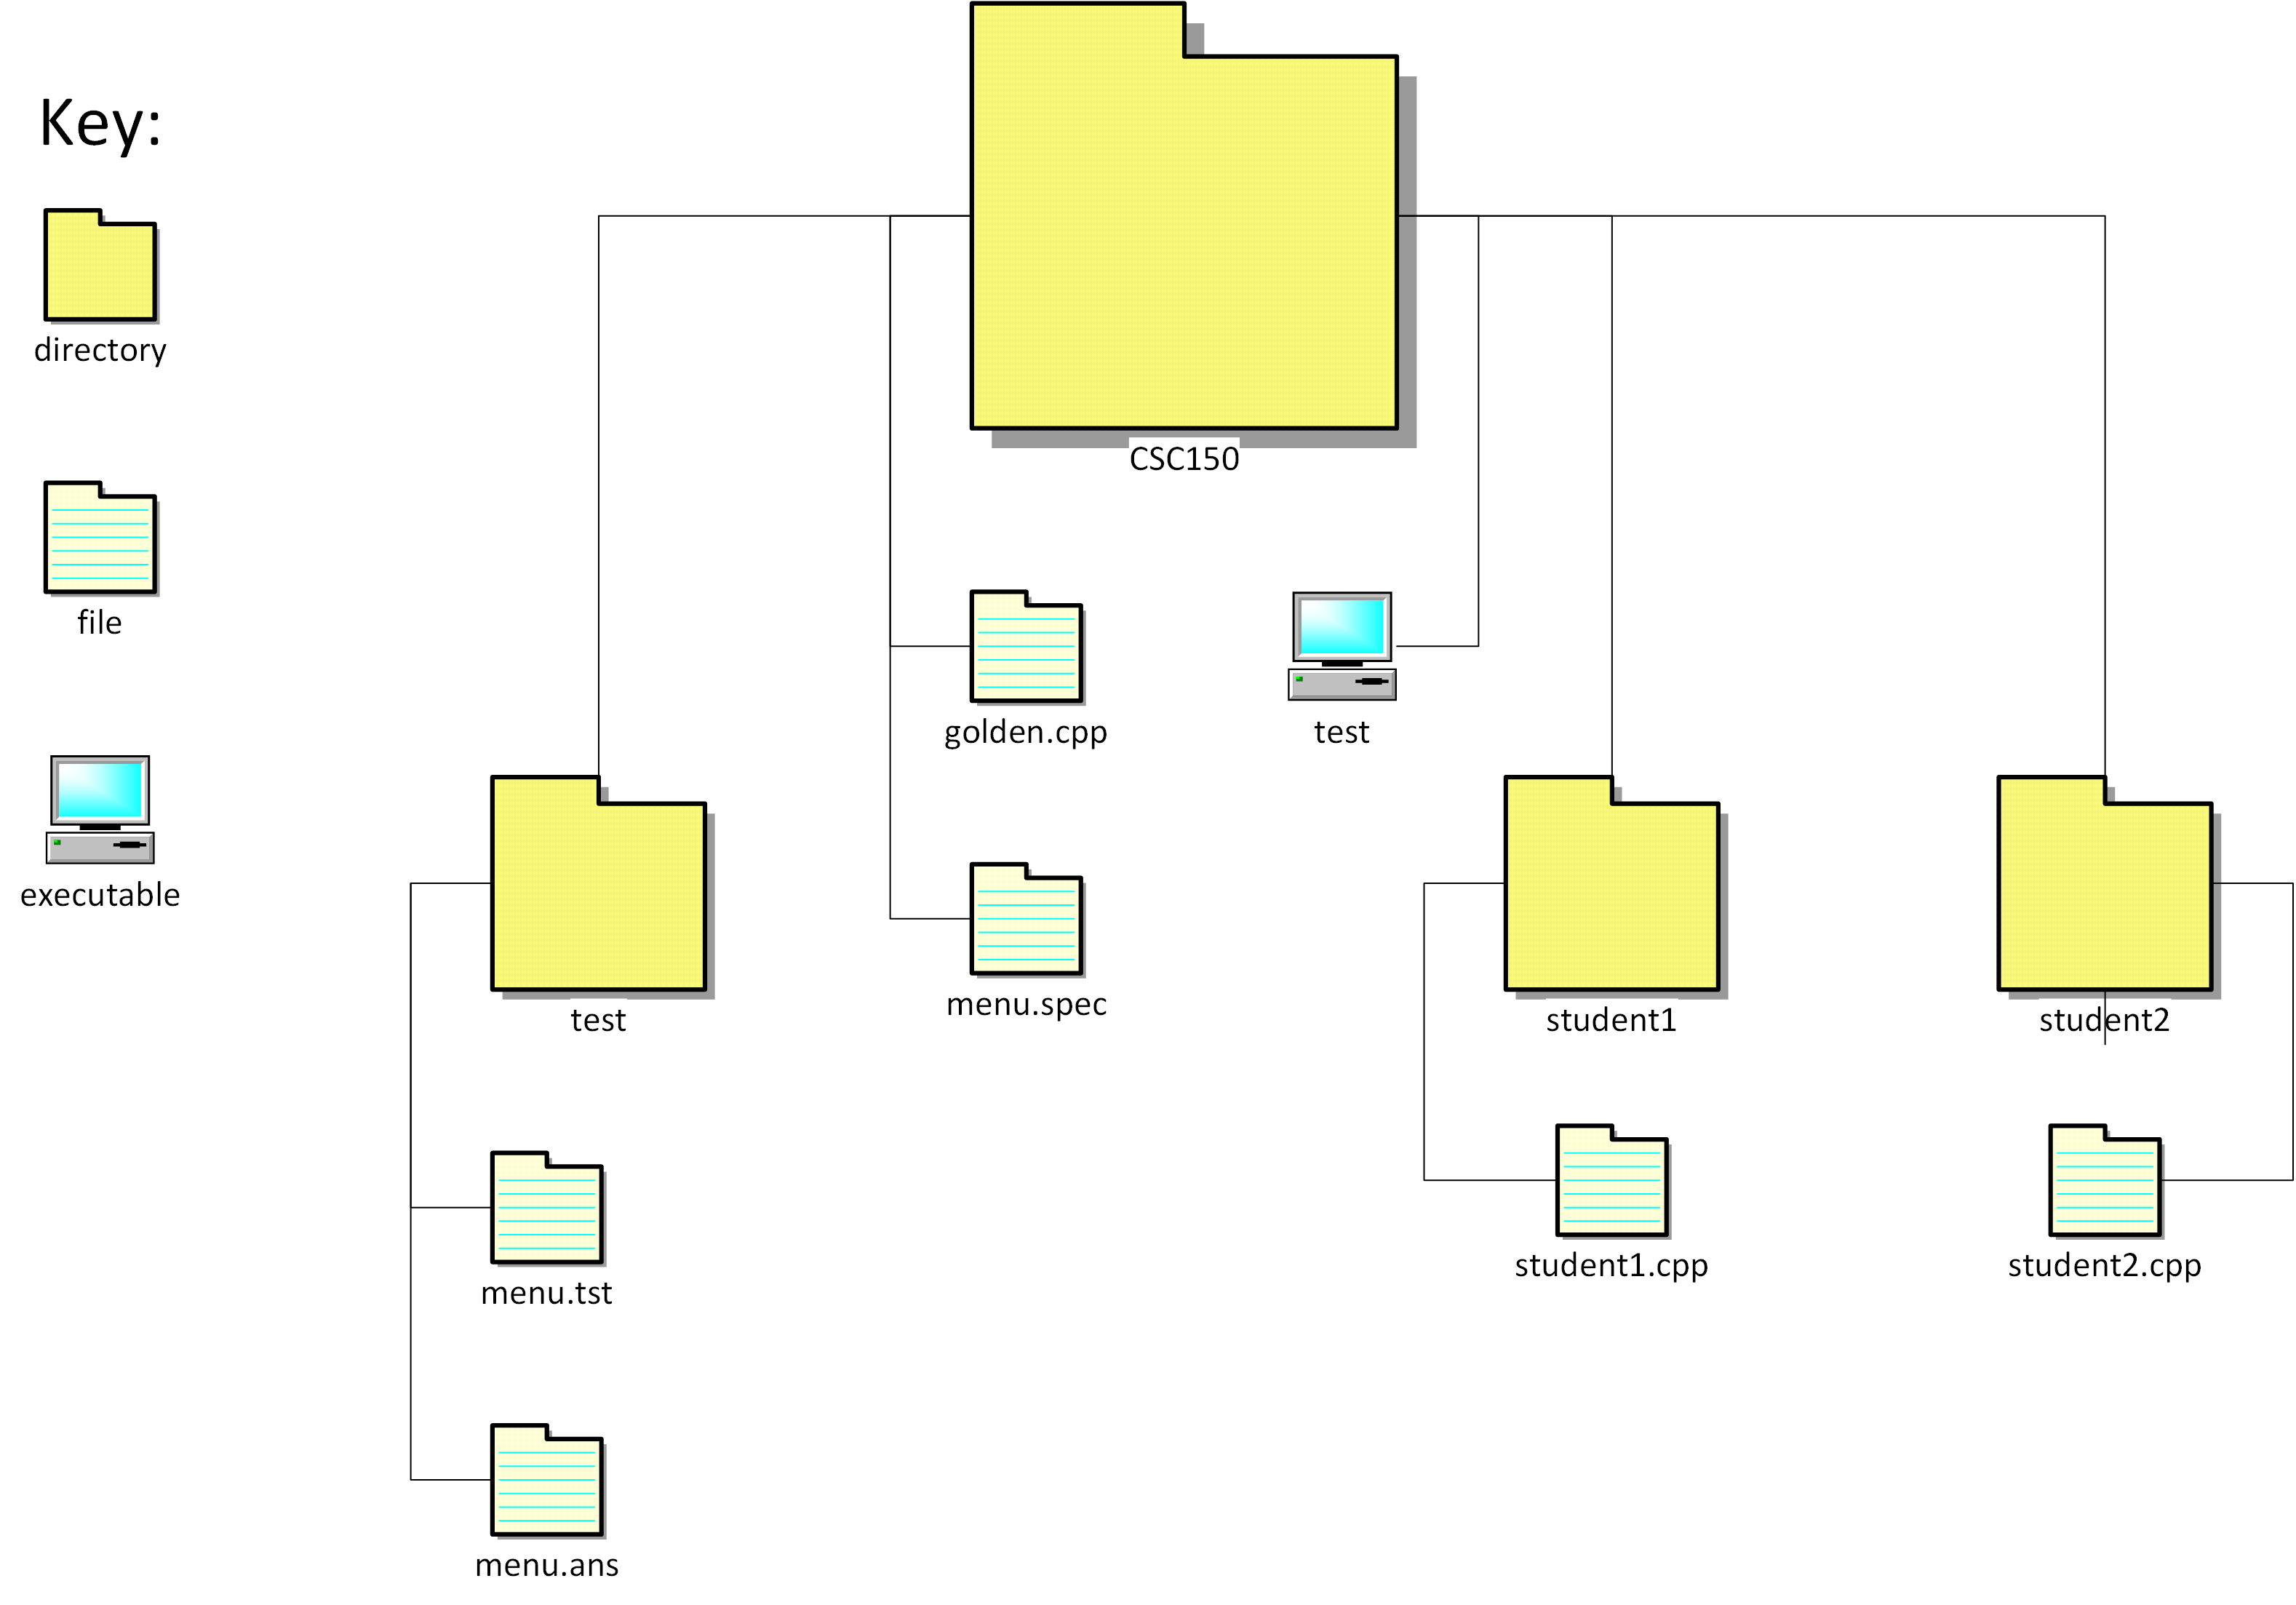
\includegraphics[width=0.75\textwidth]{./before}
\end{center}
\caption{Before test execution \label{before}}
\end{figure}

After the program, several more files have been added. The GeneratedTests directory has been created inside of test, and contains two .tst files and corresponding .ans files. In each student directory, an executable, a log file, .gprof and .gcov files, and gmon.out (created by gprof) have been added. In the parent directory, a class log has been created sharing the name of the directory. Figure ~\ref{after} shows the ending directory structure.

\begin{figure}[tbh]
\begin{center}
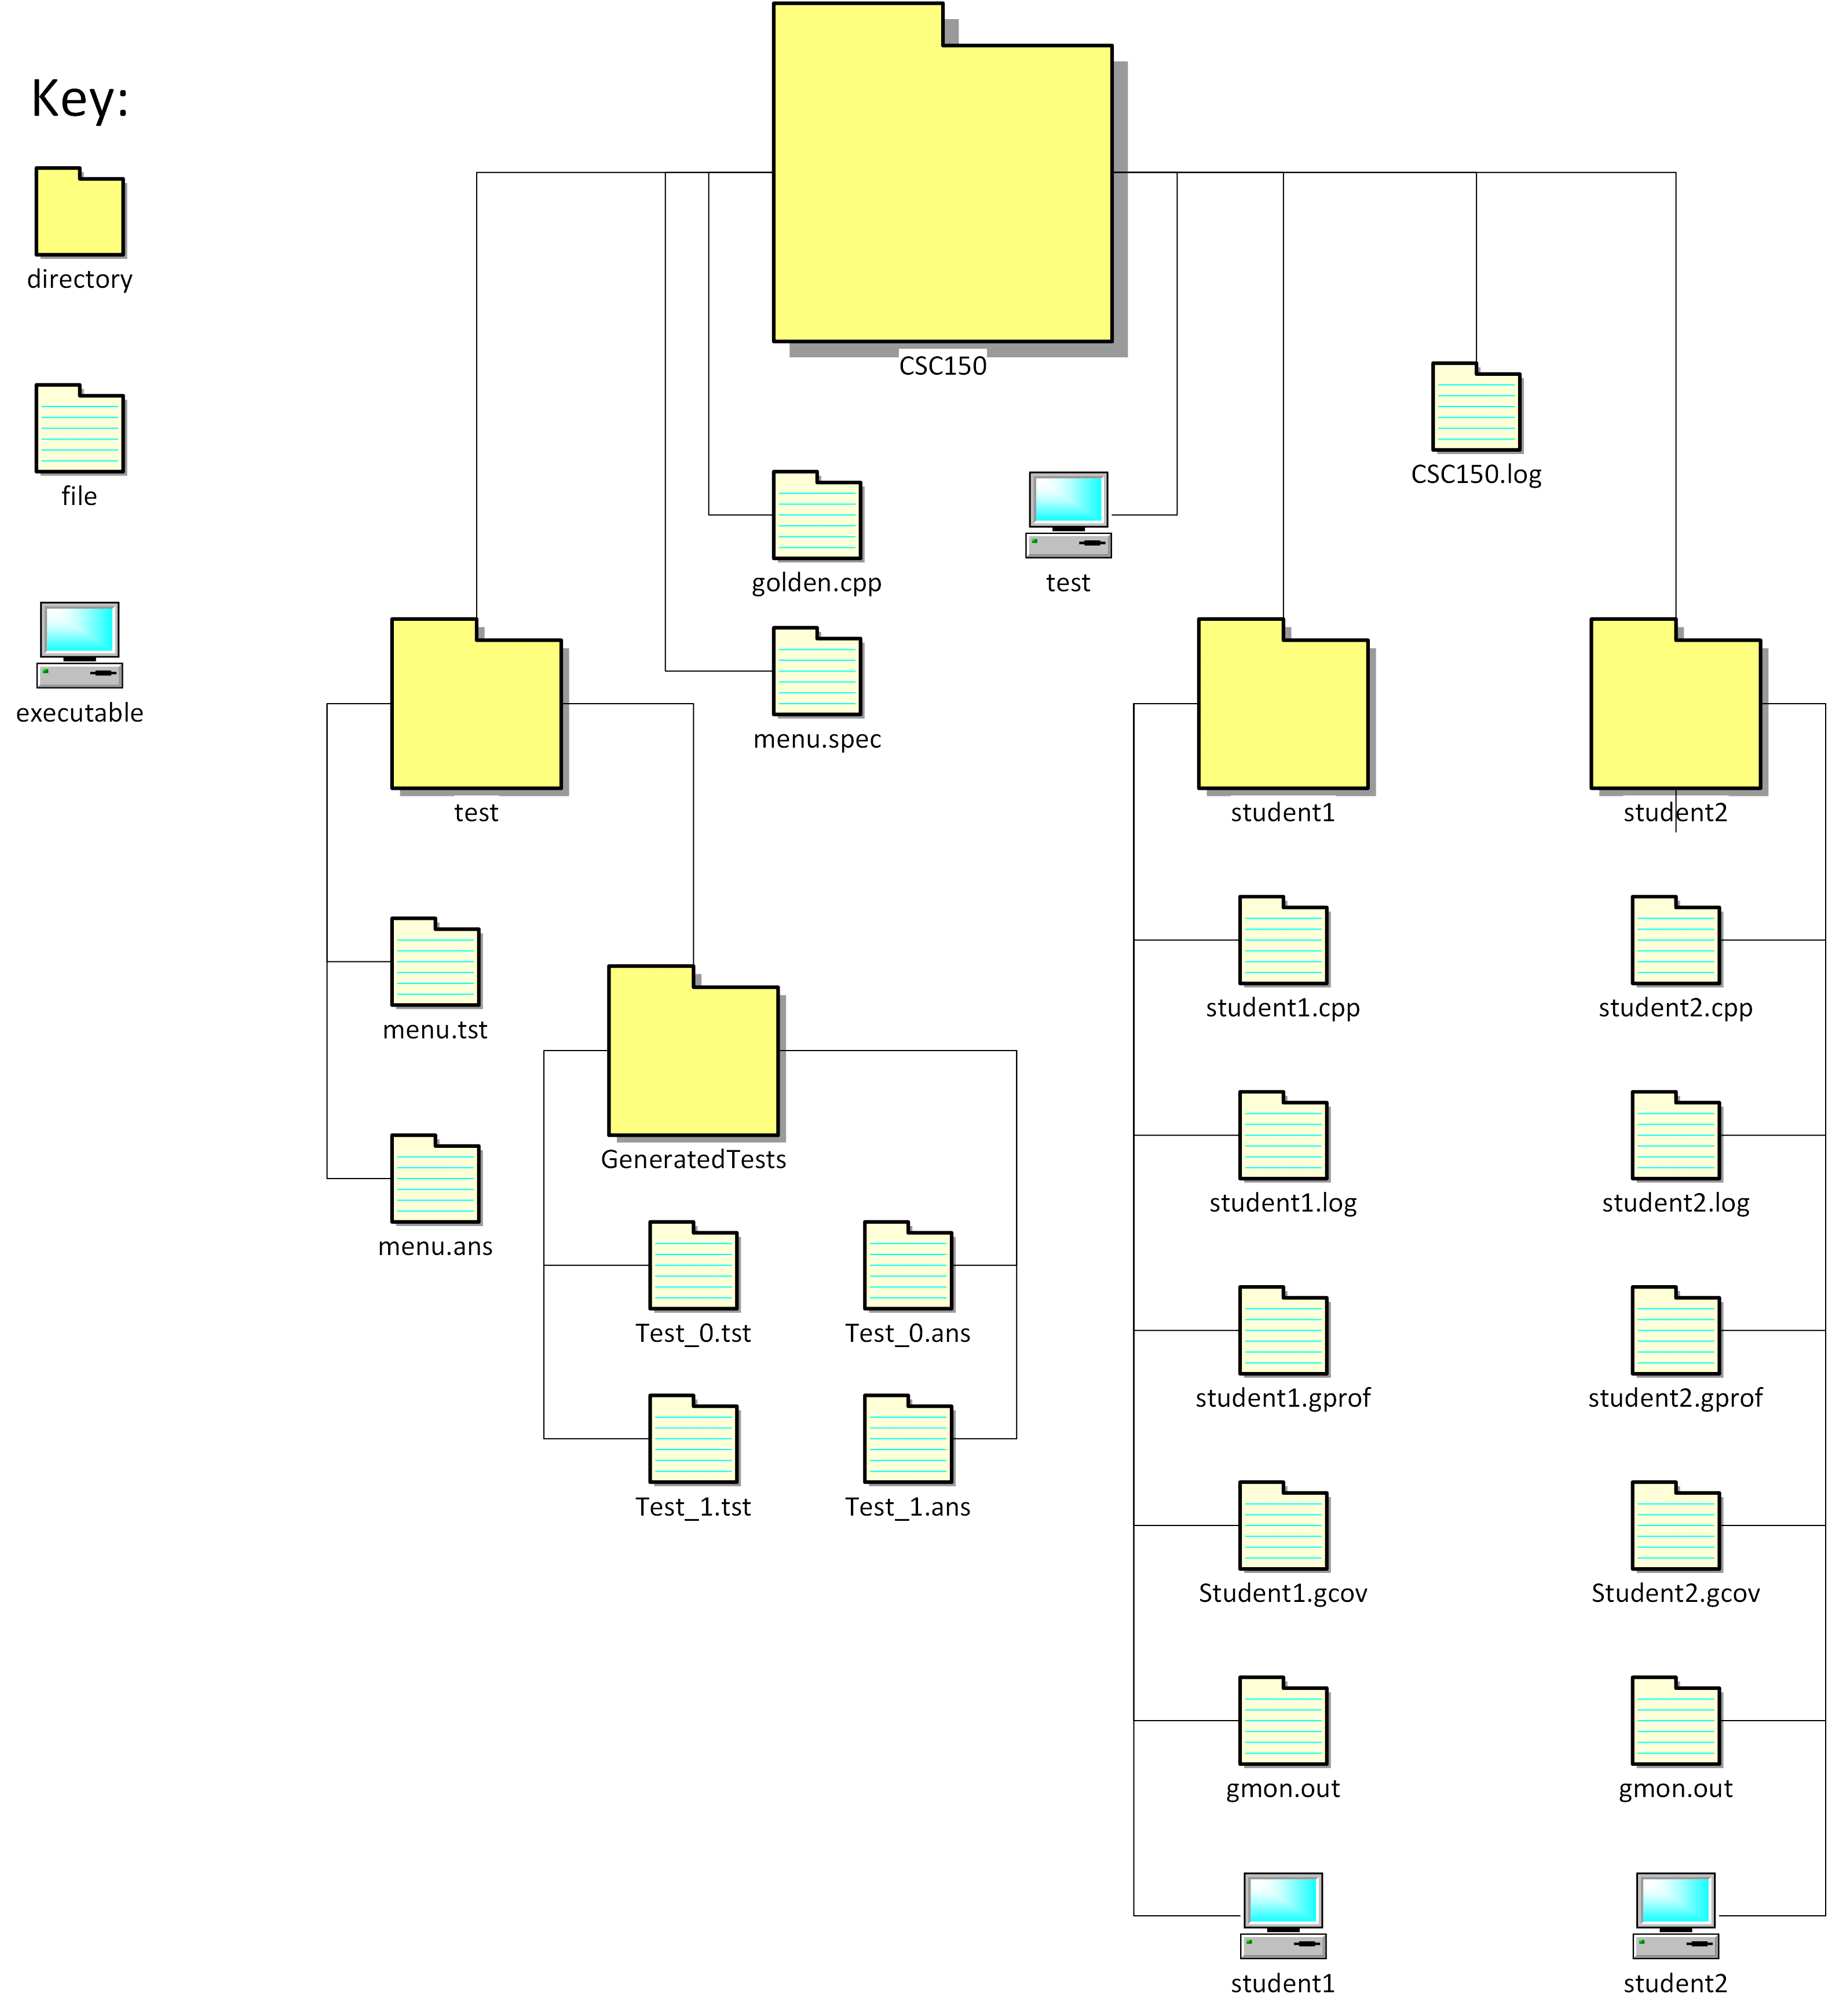
\includegraphics[width=0.75\textwidth]{./after}
\end{center}
\caption{After test execution \label{after}}
\end{figure}